\documentclass[11pt,a4paper,headinclude,footinclude,chapterprefix=on]{scrreprt} 
\usepackage[utf8]{inputenc} 
\usepackage[T1]{fontenc} 
\usepackage{tabularx} 
\usepackage{multicol} 
\usepackage{graphicx} 
\usepackage{tikz} 
\usepackage{amssymb} 
\usepackage{textcomp}

% ================================================================
% Variables
% ================================================================
\newcommand{\trnumber}{TKN-14} 
\newcommand{\trdate}{March 2014} 
\newcommand{\trauthor}{Aravinth, Sivalingam Panchadcharam} 
\newcommand{\tremail}{contact@aravinth.info} 
\newcommand{\trtitle}{Variations in Wi-Fi RSSI due to different types of Interferences}

% ================================================================
% Page Style
% ================================================================
\usepackage{geometry} \geometry{a4paper, inner=30mm, outer=25mm, top=40mm, bottom=42mm}

\usepackage[headsepline,plainheadsepline,footsepline,plainfootsepline]{scrpage2} \clearscrheadfoot

\ihead[\Large {\scshape TU Berlin }]{\Large {\scshape TU Berlin }}

\ifoot[{\tiny 
\begin{minipage}
	{4.0cm}Copyright at Technical University Berlin. 
	\newline All Rights reserved. 
\end{minipage}
}]{{\tiny 
\begin{minipage}
	{4.0cm}Copyright at Technical University Berlin. 
	\newline All Rights reserved. 
\end{minipage}
}} \cfoot[\scriptsize \trnumber]{\scriptsize \trnumber} \ofoot[Page 
\pagemark]{Page 
\pagemark}

\pagestyle{scrheadings}

\usepackage{mathptmx} 
\usepackage[scaled=.92]{helvet} 
\usepackage{courier}

\addtokomafont{pagefoot}{\normalfont}

% ================================================================
% ================================================================
\begin{document}

\bibliographystyle{plain}

% ================================================================
% Cover Sheet
% ================================================================
{ \sffamily

\thispagestyle{empty} 
\begin{tabularx}
	{\columnwidth}{cXc} 
	
\includegraphics[height=1cm]{Images/TU-Logo-3D-rot.pdf} & & 
	
\includegraphics[height=1cm]{Images/tknlogo.pdf} \\
\end{tabularx}

\vspace{1.0cm} 
\begin{center}
	{\huge 
	\noindent Technical University Berlin
	
	\vspace{0.5cm}
	
	\noindent Telecommunication Networks Group 
	\begin{center}
		\rule{15.5cm}{0.4pt} 
	\end{center}
	} 
\end{center}
\begin{minipage}
	[][11.0cm][c]{14.5cm} {\Huge 
	\begin{center}
		\trtitle 
	\end{center}
	\begin{center}
		\trauthor \\
		{\Large \tremail} 
	\end{center}
	\begin{center}
		Berlin, \trdate 
	\end{center}
	
	\vspace{0.5cm}
	
	}
	
	%\begin{center}
	%\setlength{\fboxrule}{2pt}\setlength{\fboxsep}{2mm}
	%\fbox{TKN Technical Report \trnumber}
	%\end{center}
\end{minipage}

\setlength{\fboxrule}{0.4pt} \setlength{\fboxsep}{0.4pt} 
\begin{center}
	
	\rule{15.5cm}{0.4pt}
	
	\vspace{0.5cm}
	
	{\huge {Project in advanced network technologies}}
	
	\vspace{0.5cm}
	
	{\huge Supervisors: Dr. Arash Behboodi, Filip Lemic}
	
	\vspace{0.5cm} 
\end{center}
}

% ================================================================
% Abstract
% ================================================================
\begin{abstract}
	\subsection*{\abstractname} WiFi Beacon packets are transmitted periodically to announce the presence of WLAN. RSSI is Received Signal Strength Indicator which indicates the power of signal that is received at the receiver. Beacon Packet RSSI values are extensively used for ranging and localization purpose. However, RSSI value changes with various interferences, different chipsets and distance. This project work includes an implementation of a software tool to visualize the raw data obtained during the experiments and examines how these RSSI values changed by controlled interferences. 
\end{abstract}

% ================================================================
% Tableofcontents
% ================================================================
\tableofcontents

% ================================================================
% Introduction
% ================================================================
\chapter{Introduction} 
\section{Beacon Packet} In Wireless Local Area Network (WLAN) Beacon frames are transmitted periodically by Base Station Set (BSS) to announce the presence of Wi-Fi Network. Beacon frame is one of the management frames in IEEE 802.11. Figure \ref{fig:beacon} shows the fields of Beacon frame.

\begin{figure}
	[!h] \centering 
	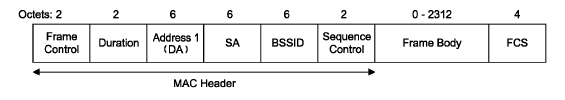
\includegraphics[width=15cm]{Images/beacon_frame.png} \caption{MPDU - Beacon Frame of IEEE 802.11} \label{fig:beacon} 
\end{figure}

\section{Received Signal Strength Indicator (RSSI)} RSSI is an indication of the power level received by a receiver expressed in dBm. RSSI is a generic radio receiver technology metric, which is usually invisible to the user of the device containing the receiver, but is directly known to users of wireless networking of IEEE 802.11 protocol family. RSSI can be used internally in a wireless networking card to determine when the amount of radio energy in the channel is below a certain threshold at which point the network card is clear to send (CTS). Once the card is clear to send, a packet of information can be sent. RSSI is generally visible to the user in the form of signal strength as shown in the Figure \ref{fig:rssi} 

\begin{figure}
	[!h] \centering 
	
\includegraphics[width=8cm]{Images/rssi.png} \caption{Signal Strength Indicator in Wireless devices } \label{fig:rssi} 
\end{figure}

% ================================================================
% Problem Statement
% ================================================================
\chapter{Problem Statement}
\section{Accuracy}
Different studies show that RSSI values have significant variations due to various factors.
\begin{itemize}
\item RSSI values are reported significantly different by different hardwares.
\item RSSI values vary with change in temperature.
\item RSSI values are affected by various interferences.
\item The relation between RSSI values and distance between
transmitter and receiver is unreliable.
\end{itemize}

\begin{figure}
	[!h] \centering 
	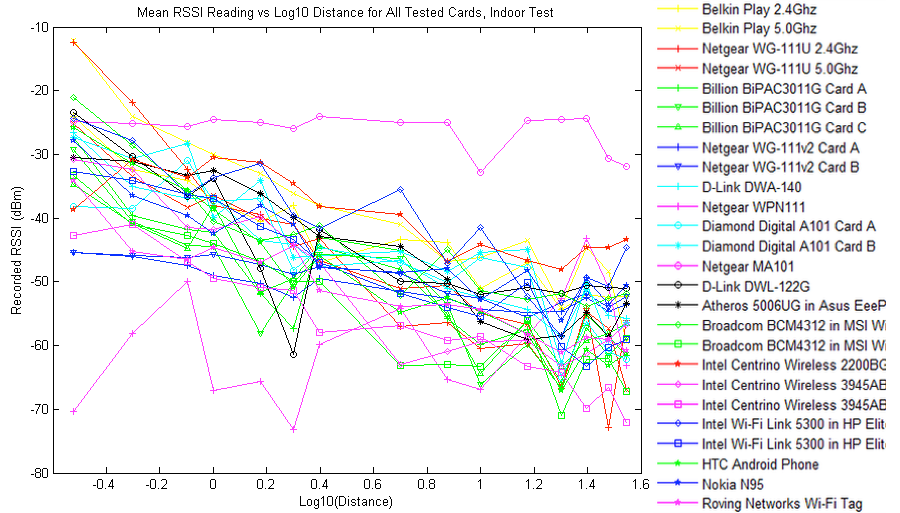
\includegraphics[width=15cm]{Images/rssi_vendor1.png} \caption{RSSI values recorded from different hardwares} \label{fig:rssi_vendors} 
\end{figure}

\section{Standardization}
There is no standardized relationship of any particular physical parameter to the RSSI reading. The 802.11 standard does not define any relationship between RSSI value and power level in mW or dBm. Vendors and chipset makers provide their own accuracy, granularity, and range for the actual power (measured as mW or dBm) and their range of RSSI values (from 0 to RSSI Max). Figure \ref{fig:rssi_vendors} shows the variance of RSSI values due to different hardwares and vendors.

\section{RSSI in Indoor Localization}
RSSI is also extensively used for RF based ranging and localization purposes. It is then used to estimate the distance between
transmitter and receiver. The physics behind this technology
is the power level decay with distance. 

\section{Interferences}
Due to the reason that RSSI is used for other purposes where the accuracy and reliability should be guaranteed, few experiments were carried out as a part of this project work to analyze the change in RSSI values due to various interferences. Following sections describe about it clearly.

% ================================================================
% RSSI Visualization Tool
% ================================================================
\chapter{Raw Ranging Data Visualization Tool}
\section*{Introduction} 
Measurements yield large amount of raw data which contains the complete information of experiments such as testbed measurement locations, access points, rssi, channel, ssid, bssid, latency. In order to track collected raw data, a raw ranging data visualization tool was implemented. 

\paragraph{}This tools helps us to list and visualize the available databases and collections of experiments under one hood. It is a web-based standalone software which was implemented using Javascript and various libraries. This tool can be simply started by opening it on a web browser. It needs an Internet connection to retrieve data from the backend servers. It makes use of asynchronous (AJAX) ability of Javascript and processes large array of raw data. This tool consists of 4 panels which showcases the work flow in an user friendly manner. Usage and functionality of each panel is explained in the following sections.

\begin{figure}
	[!h] \centering 
	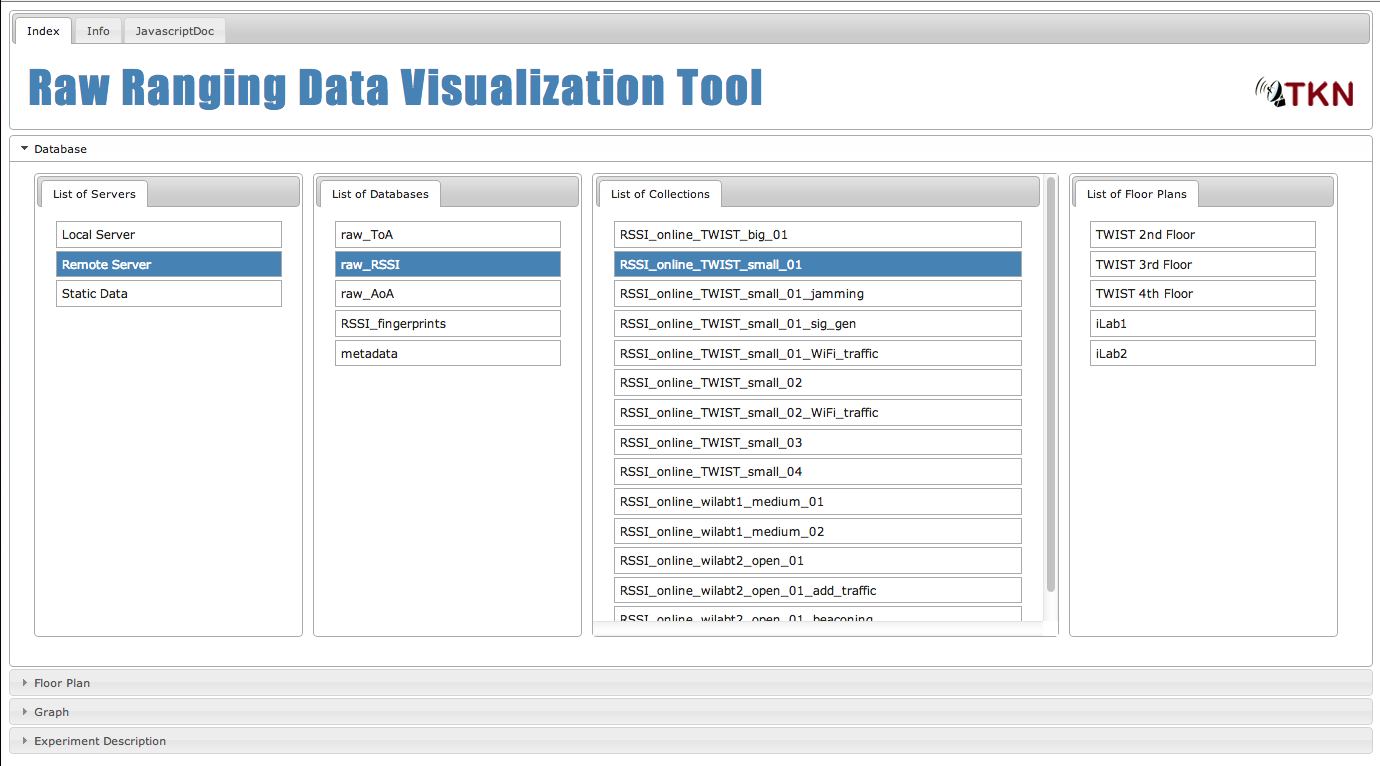
\includegraphics[width=15cm]{Images/tool_db.png} \caption{Dashboard of the visualization tool} \label{fig:tool:db} 
\end{figure}
 
\section{Dashboard} 
Figure \ref{fig:tool:db} shows the Dashboard panel that is the landing page of this tool. It contains 4 sub-panels. 

\begin{description}
\item[List of Servers] lists URIs of server that contains various RAW data collected from the experiments. Remote Server contains the complete set of RAW data. Copy of the RAW data can also be stored on the local machine. Static Data contains a simple set of RAW data for the purpose of debugging. 
\item[List of Databases] lists URIs of databases which are stored in the server. 
\item[List of Collections] lists the collections of experiments which were carried out. URI denotes the name of Testbed, experiment size and experiment type.
\item[List of Floor Plans] lists the names of the floor plans on which experiments were carried out. Floor Plan must be selected according to the experiment. 
\end{description}

\begin{figure}
	[!h] \centering 
	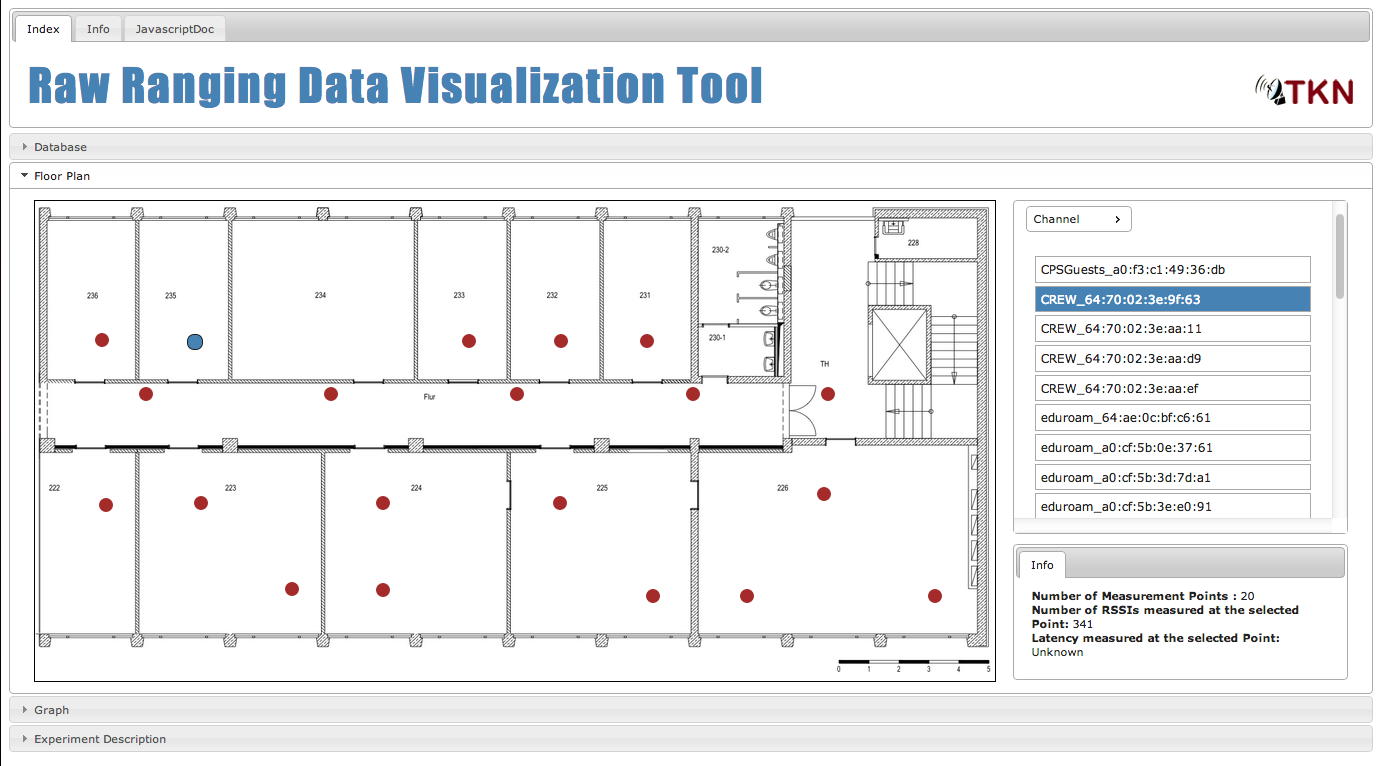
\includegraphics[width=15cm]{Images/tool_floor.png} \caption{Floor Plan of the visualization tool} \label{fig:tool:floor} 
\end{figure}

\section{Floor Plan} 
Figure \ref{fig:tool:floor} shows Floor Plan panel that contains the map of selected testbed. Once the appropriate floor plan for an experiment is selected, all the measurement points are loaded into the map. Measurement point is circular button that turns blue when it is clicked and it lists RSSI values measured at that geographical point. On the right side of the Floor Plan, Channel and SSID information of the selected measurement point is shown. If the Raw Data contains channel information, then it will be listed in the dropdown other it will be listed as Unknown. RSSI values are grouped together on the basis of same SSID and BSSID. Info tab at the right below shows some specific information about the selected measurement point.

\begin{figure}
	[!h] \centering 
	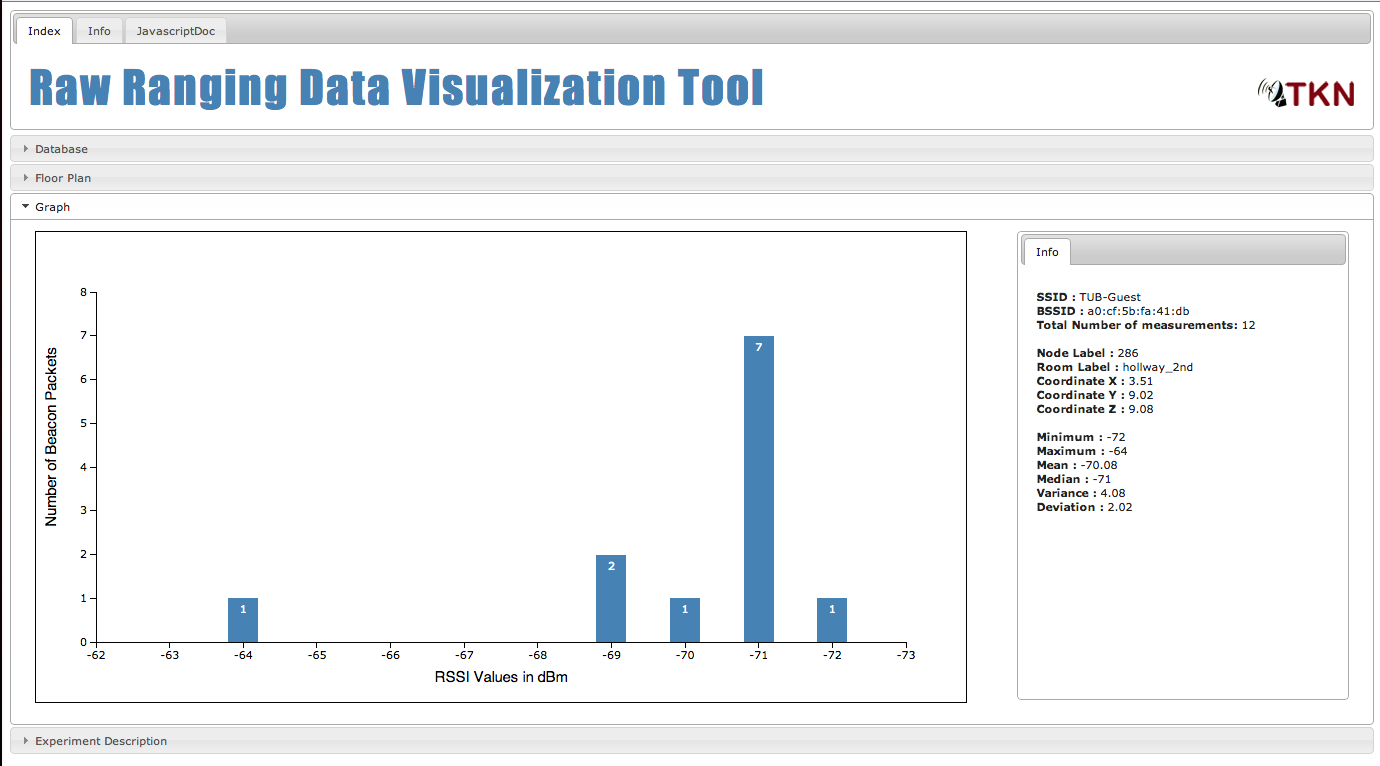
\includegraphics[width=15cm]{Images/tool_graph.png} \caption{Graph of the visualization tool} \label{fig:tool:graph} 
\end{figure}

\section{Graph} 
Figure \ref{fig:tool:graph} shows Graph panel that contains a histogram that is generated dynamically by selecting a particular access point on Floor Plan panel. Number of Bins of the histogram are also dynamically adjusted based on the total number of RSSI values measured. Info tab shows coordinate information of the selected measurement points as well as the statistics of RSSI values.

\begin{figure}
	[!h] \centering 
	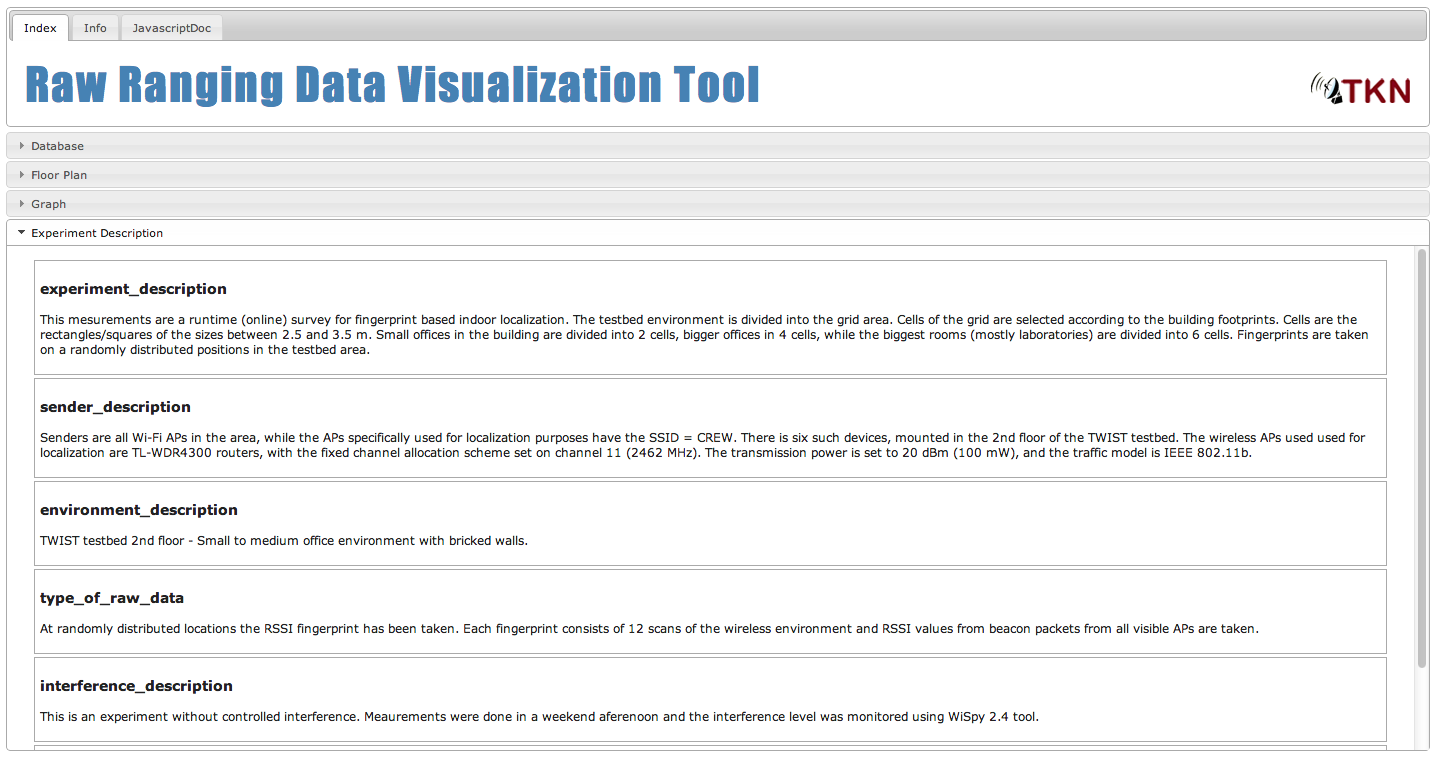
\includegraphics[width=15cm]{Images/tool_des.png} \caption{Experiment Description of the visualization tool} \label{fig:tool:des} 
\end{figure}

\section{Experiment Description} 
Figure \ref{fig:tool:des} shows Experiment Description panel that contains detail of the experiment such as testbed environment, sender and receiver device specification and interference pattern. This information is stored in Metadata database. 

\begin{figure}
	[!h] \centering 
	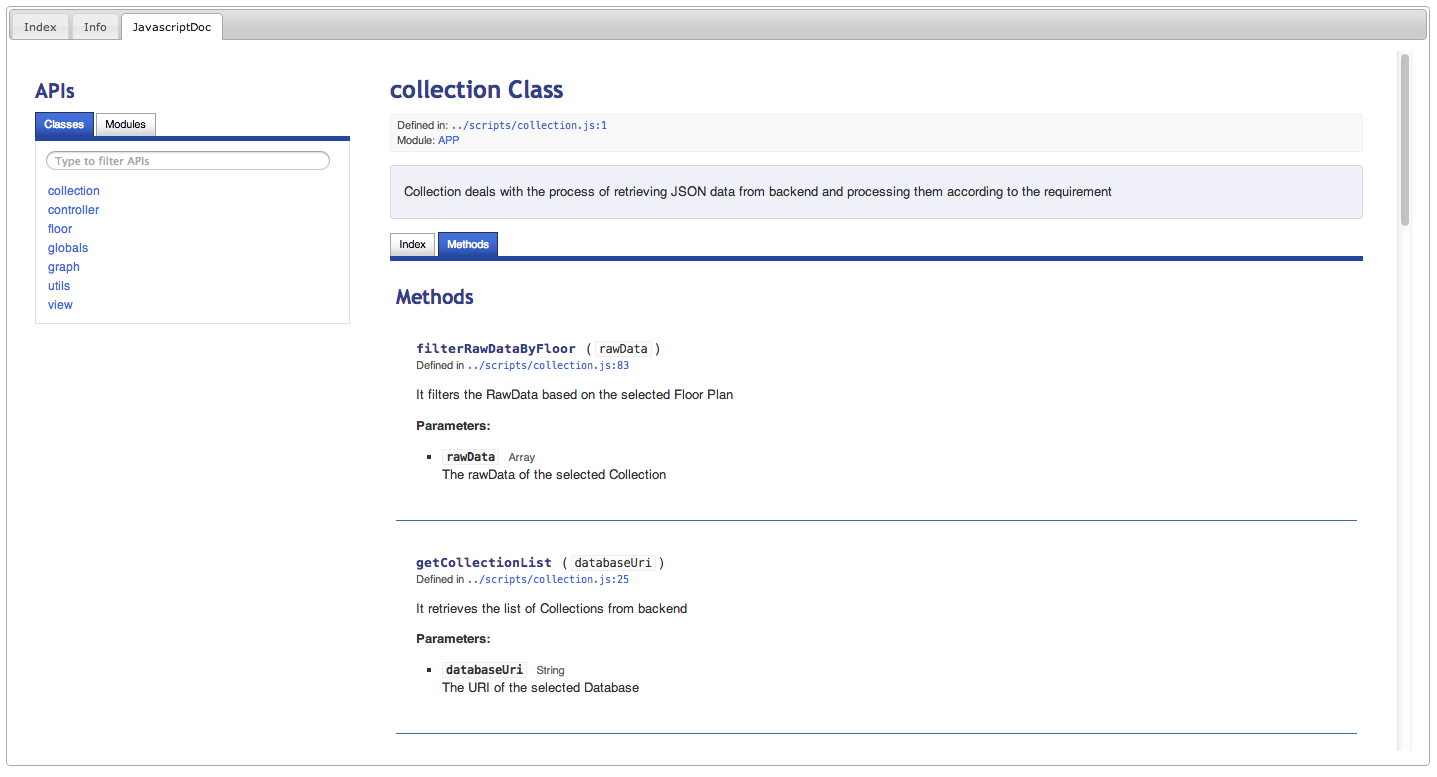
\includegraphics[width=15cm]{Images/tool_jsDoc.png} \caption{API of the visualization tool} \label{fig:tool:jsDoc} 
\end{figure}

\section{API} 
Figure \ref{fig:tool:jsDoc} shows API that is a Javascript documentation which can be viewed by clicking on JavascriptDoc button on the top menu. API reveals the Functions, Constants, Views, Collections, Events and Utilities used to visualize the Raw Ranging Data. It helps to extend this program, do further implementation, add new features and debug the code. 

% ================================================================
% Design
% ================================================================
\chapter{Design} 
\section{Reference Scenario} 
This reference scenario is instantiated on the 2nd floor of the TWIST testbed. It is called “Reference scenario” because no artificial interference is generated and the presence of uncontrolled interference is minimized. According to the EVARILOS Benchmarking Handbook (EBH), this scenario is an instance of the “Small office” type of scenarios. In this scenario 20 measurement points are defined and their locations are given in Figure \ref{fig:floor}.

\begin{figure}
	[!h] \centering 
	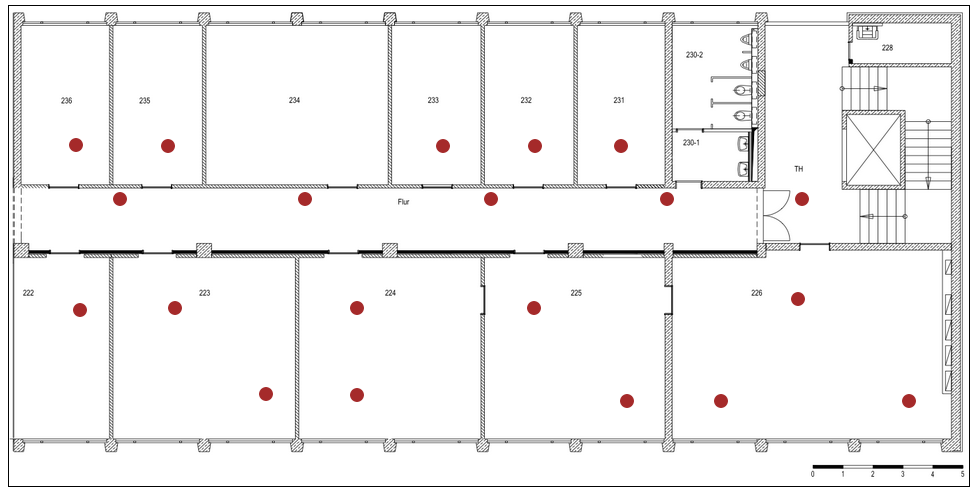
\includegraphics[width=100mm]{Images/floor} \caption{Locations of measurement points} \label{fig:floor} 
\end{figure}

\paragraph{} At each measurement point the indoor localization System Under Test (SUT) is requested to estimate location. The SUT device is carried to each measurement location using the robotic platform. The navigation stack of the robotic platform gives one order of magnitude more accurate location estimation than considered SUTs and the location obtained from the robotic platform is considered as the ground truth.

\paragraph{} The experiments were performed at the weekend afternoon, so the influence of interferes has been minimized. Furthermore, the wireless spectrum has been measured using the WiSpy device attached to the robotic platform and all measurements with the interference threshold above certain level have been repeated. Finally, before each experiment a more detailed measurement of the spectrum has been taken with the spectrum analyzer at a predefined location.

\section{Interference Scenarios}\label{sec:interference}
\subsection{Interference Scenario 1} First interference scenario instantiated in TWIST testbed uses the testbed Wireless Fidelity (WiFi) nodes as interference sources. Interference type is jamming on one IEEE 802.11 channel with the maximum transmission power. Three of such jamming nodes are present at different locations in the testbed environment. Summary of this interference scenario is given in Table \ref{tb:interf:1}.
\begin{table}
	[h] \centering \caption{Interference scenario summary} \label{tb:interf:1} 
	\begin{tabular}
		{|l|l|} \hline \multicolumn{2}{|c|}{Types of interference sources} \\
		\hline WiFi & \checkmark \\
		Microwave & \texttimes \\
		DECT & \texttimes \\
		Bluetooth & \texttimes \\
		3G & \texttimes \\
		ZigBee & \texttimes \\
		\hline \multicolumn{2}{|c|}{Types of interference sources} \\
		\hline Number of sources & 3 \\
		Power & 20 dBm \\
		Waveform & Carrier jamming \\
		Specific pattern & \\
		Start \& stop time & Beginning \& end of experiment \\
		Traffic model & \\
		\hline \multicolumn{2}{|c|}{Traffic parameters of interference} \\
		\hline Packet size & \\
		Inter-packet gap & \\
		Bit rate & \\
		File size & \\
		Start \& stop size & \\
		Traffic model & \\
		\hline \multicolumn{2}{|c|}{Network parameters} \\
		\hline Network size & \\
		Node density & \\
		Node mobility & \\
		Node failures & \\
		\hline 
	\end{tabular}
\end{table}

\subsection{Interference Scenario 2}In this interference scenario instantiated in TWIST testbed interference is created using the IEEE 802.15.4 Tmote Sky nodes. The interference type is jamming on one IEEE 802.15.4 channel with a constant transmit power equal to 0 dBm. Five of these jamming nodes will be present in the testbed environment. Summary of this interference scenario is given in Table \ref{tb:interf:2}.
\begin{table}
	[h] \centering \caption{Interference scenario summary} \label{tb:interf:2} 
	\begin{tabular}
		{|l|l|} \hline \multicolumn{2}{|c|}{Types of interference sources} \\
		\hline WiFi & \texttimes \\
		Microwave & \texttimes \\
		DECT & \texttimes \\
		Bluetooth & \texttimes \\
		3G & \texttimes \\
		ZigBee & \checkmark \\
		\hline \multicolumn{2}{|c|}{Types of interference sources} \\
		\hline Number of sources & 5 \\
		Power & 0 dBm \\
		Waveform & Carrier jamming \\
		Specific pattern & \\
		Start \& stop time & Beginning \& end of experiment \\
		Traffic model & IEEE 802.15.4 radio \\
		\hline \multicolumn{2}{|c|}{Traffic parameters of interference} \\
		\hline Packet size & \\
		Inter-packet gap & \\
		Bit rate & \\
		File size & \\
		Start \& stop size & \\
		Traffic model & \\
		\hline \multicolumn{2}{|c|}{Network parameters} \\
		\hline Network size & \\
		Node density & \\
		Node mobility & \\
		Node failures & \\
		\hline 
	\end{tabular}
\end{table}

\subsection{Interference Scenario 3}Second interference scenario instantiated in TWIST testbed defines interference types that is usual for the office and home environments. Namely, interference is emulated using 4 WiFi embedded Personal Computers (PCs), namely a server, email client, data client, and video client. The server acts as a WiFi Access Point (AP) and a gateway for the emulated services. The email client will “check email” once every 15 seconds for a duration of one second. The data client is emulated via TCP streams one starting at 45 seconds for a duration of 22.5 seconds and the other starting at 105 seconds for a duration of 45 seconds. The video client is emulated as a UDP stream of 100 kbps for half the experiment cycle and it will start at the middle of the experiment. In total, the experiment takes 150 seconds. Summary of this interference scenario is given in Table \ref{tb:interf:3}.
\begin{table}
	[h] \centering \caption{Interference scenario summary} \label{tb:interf:3}
	\begin{tabular}
		{|l|l|} \hline \multicolumn{2}{|c|}{Types of interference sources} \\
		\hline WiFi & \checkmark \\
		Microwave & \texttimes \\
		DECT & \texttimes \\
		Bluetooth & \texttimes \\
		3G & \texttimes \\
		ZigBee & \texttimes \\
		\hline \multicolumn{2}{|c|}{Types of interference sources} \\
		\hline Number of sources & 3 \\
		Power & 20 dBm \\
		Waveform & \\
		Specific pattern & \\
		Start \& stop time & Beginning \& end of experiment \\
		Traffic model & WiFi traffic \\
		\hline \multicolumn{2}{|c|}{Traffic parameters of interference} \\
		\hline Packet size & \\
		Inter-packet gap & \\
		Bit rate & \\
		File size & \\
		Start \& stop size & \\
		Traffic model & \\
		\hline \multicolumn{2}{|c|}{Network parameters} \\
		\hline Network size & \\
		Node density & \\
		Node mobility & \\
		Node failures & \\
		\hline 
	\end{tabular}
\end{table}

% ================================================================
% Experiments
% ================================================================
\chapter{Experiments} 
\section{Infrastructure} 
Experiments are carried on two different Testbeds. As shown in the figure \ref{fig:experiment}, Testbeds provide a robotic automated platform to carry out the experiment. Setting up the measurement points, configuring the nodes, accessing signal generators and various other devices are done with the help of control center. 

\begin{figure}
	[!h] \centering 
	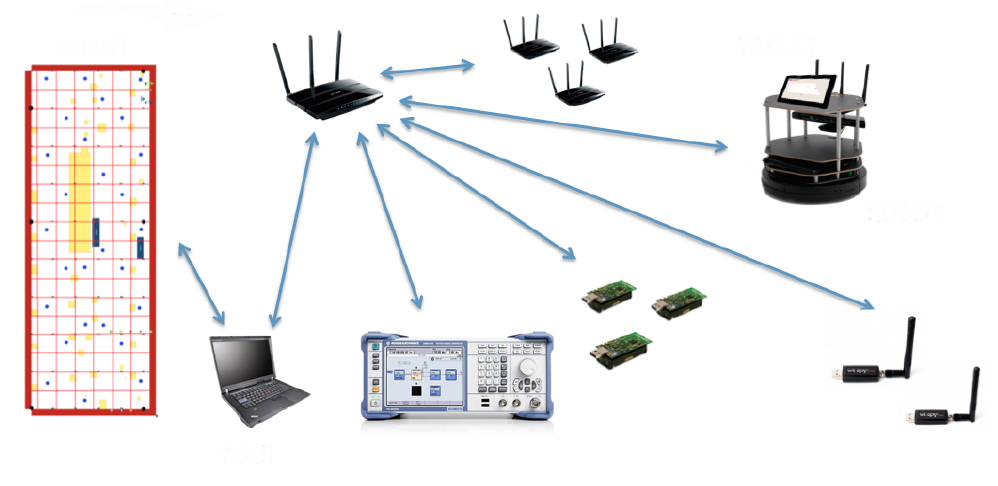
\includegraphics[width=15cm]{Images/evari.png} \caption{Experiment Environment} \label{fig:experiment} 
\end{figure}

\section{Testbed}
\subsection{TWIST}
The TKN Wireless Indoor Sensor network Testbed (TWIST), developed by the Telecommunication Networks Group (TKN) at the Technische Universität Berlin, is a scalable and flexible testbed architecture for experimenting with wireless sensor network applications in an indoor setting. It provides basic services like node configuration, network-wide programming, out-of-band extraction of debug data and gathering of application data.

It is equipped with 102 TmoteSky nodes and 102 eyesIFX nodes. For the experiments 3 Different Floor Plans are used. Signal Generators are used to generate microwave signals which were used to jam the channel during the experiments. From control center fixed coordinates
are set to the robot, so that accurate measurement points are achieved in the experiments. 

\subsection{iLab.t}
The iMinds iLab.t technology centre offers the experimentation environments, the hardware, the measurement equipment and the software tools needed to develop your ICT innovations, and/or test their performance and service quality.

A generic experimentation facility of 100 nodes (dual processor, dual core servers) interconnected via non-blocking 1.5 Tb/s Ethernet switch, called the Virtual Wall. Two generic wireless experimentation facilities of 200 and 80 nodes respectively, specifically targeting innovations involving the use, configuration or set-up of wireless networks (includes Wi-Fi, 802.15.4, Bluetooth, sensor nodes, mobile robots and a mobility emulation set-up), called the w-iLab.t.

\section{Experiment Procedure}
This shows step by step how experiments were carried out. 
\begin{itemize}
\item Measurement points of testbed are loaded into the Robot. 
\item System Under Test (SUT) is equipped with Network Interface Card (NIC) and loaded with program to store RSSI, SSID, BSSID, Latency values.
\item SUT is placed on the top of the Robot.
\item Robot is commanded from the control center to move to the first measurement point.
\item SUT is commanded to start the measurement.
\item SUT scans the Wireless Spectrum in the environment for WiFi Access Points and stores RSSI, SSID, BSSID, Latency values. This step is iterated 20 times.
\item Measurements are stored on cloud database.
\item Robot moves to other measurement point and repeats the above given steps‚
\end{itemize}

\section{Reference Scenario Experiment}
Since this experiment is conducted under environment where no artificial interference is generated and the presence of uncontrolled interference is minimized, this experiment is referred to as reference scenario. Experiments with controlled interferences are carried out in the similar way with artificially generated interferences. Section \ref{sec:interference} shows the details of various interferences which were generated during the experiments.


\subsection{Experiment Description}
This mesurements are a runtime (online) survey for fingerprint based indoor localization. The testbed environment is divided into the grid area. Cells of the grid are selected according to the building footprints. Cells are the rectangles/squares of the sizes between 2.5 and 3.5 m. Small offices in the building are divided into 2 cells, bigger offices in 4 cells, while the biggest rooms (mostly laboratories) are divided into 6 cells. Fingerprints are taken on a randomly distributed positions in the testbed area.

\subsection{Environment Description}
TWIST testbed 2nd floor - Small to medium office environment with bricked walls.

\subsection{Sender Description}
Senders are all Wi-Fi APs in the area, while the APs specifically used for localization purposes have the SSID = CREW. There is four such devices, mounted on the corners of the 2nd floor of the TWIST testbed. The wireless APs used used for localization are TL-WDR4300 routers, with the fixed channel allocation scheme set on channel 11 (2462 MHz). The transmission power is set to 20 dBm (100 mW), and the traffic model is IEEE 802.11b.

\subsection{Receiver Description}
Receiver is a MacBook Pro notebook with the AirPort Extreme network interface card (NIC).

\subsection{Raw Data}
At randomly distributed locations the RSSI fingerprint has been taken. Each fingerprint consists of 20 scans of the wireless environment and RSSI values from beacon packets from all visible APs are taken.

\subsection{Interference Description}
This is an experiment without controlled interference. Measurements were done in a weekend afternoon and the interference level was monitored using WiSpy 2.4 tool.


% ================================================================
% Results
% ================================================================
\chapter{Analysis}
\section{Spatial Distribution}
Spatial Distribution of mean value of RSSIs shows the strength of RSSI values in the geometrical plane of Floor Plan.

\section{Repeatability}
\subsection{Repeatability Condition}
It is defined as a condition where independent test results are obtained with the same method on identical test items in the same laboratory by the same operator using the same equipment within short intervals of time.

In our case, it is defined as a condition which satisfies the following:
\begin{itemize}
\item Same Testbed
\item Same Laboratory (Floor)
\item Same Measurement point
\item Same Channel
\item Same Sender (SSID and BSSID)
\end{itemize}

An experiment which satisfies this condition is called as cell. 

\subsection{Repeatability}
Repeatability is precision under repeatability condition that describes the minimum variability in results.

\begin{equation}\label{eq:variance}
{S}_i^2 = {\sigma}^2 =  \frac{\sum\limits_{i=1}^{n} (x_{i} - \bar{X}^2)}{n-1}
\end{equation}

In equation \ref{eq:variance},
 $S_{i}^{2}$ is the variance of each cell, where each cell is test results of experiment that satisfies the repeatability condition, $(x_{i} - \bar{X}^2)$ is the difference from the mean value and $n$ is total number of values in the set.

\begin{equation}\label{eq:repeat}
{S}_r^2 = \frac{\sum\limits_{i=1}^{n} (n_{i} - 1){S}_i^2}
{\sum\limits_{i=1}^{n}(n_{i} - 1)}
\end{equation}

In equation \ref{eq:repeat},
${S}_r^2$ is repeatability variance, n is total number of repetition of cell, $S_{i}^{2}$ is the variance of each cell. 


% ================================================================
% Conclusion
% ================================================================
\chapter{Results}

% ================================================================
% Conclusion
% ================================================================
\chapter{Conclusion}

\pagebreak 

\begin{thebibliography}
	{9} \bibitem{lamport94} Ref1 
\end{thebibliography}

\end{document} 
